\chapter{The Case}
%Development
Since no library with Android support currently exist it was decided to use the Motej library as a core for further development.

\section{Introduction}
At the time of writing no research has been done on using motion game controllers as peripherals in a smart-phone based bio-feedback system. In order to answer the research questions posed in this report it will be necessary to create a simple but working prototype of the aforementioned system. The equipment used to realize the system will be a rooted HTC Desire HD \cite{desireHdSpecs} running CyanogenMod 7 and Wii Remotes with the Motion Plus extension. The application will be created using the Android SDK, Java and the Motej library.


%Write about why we chose motej?

\section{Software Architecture}
In this section contains an explanation and documentation of the various software architectural choices.

The two main focuses when creating the architecture was \emph{modifiability} and \emph{usability}. Modifiability was important to insure the ability to replace the Wii remote with other senors without major changes in the source code. Though the main goal of this project does not include the creation of a complex graphical user interface, usability was still considered a priority for the source code to be reused in future work. 

\subsection{Architectural Patterns}
\subsubsection{Event-driven architecture}
Event-driven architecture is an architectural pattern that focuses on the creation and cosumption of events. The event emitters creates new events and pushes them to the event consumers. The event consumers uses the events to produce some reaction. Because the event emitter does not directly speak with the event consumers this pattern makes the different components very loosely coupled.

In our case the event emitters will be the motej and motejx libraries. These classes will handle the connection to the Wii remote and the MotionPlus extension and create events when it receives new date from the Wii remote or its extensions. The event consumers will be the models that change the state in accordance to the received events containing the sensor data. Using this pattern the models are not concerned with the way the event emittors are implemented or what kind of sensors they connect to as long as the events emitted are on the same form.

Fortunatly Motej already implemented the event-driven architecture so there was no need to modify the library in this aspect.

\begin{lstlisting}
//Example of event-driven architecture using 
//java.swing.event.EventListenerList and 
//java.util.EventListener

//Event emittor (parts from the Mote class)
EventListenerList listenerList = new EventListenerList();
...
public void addAcceleromterListener(AcceleromterListener<Mote> listener) {
	listenerList.add(AccelertomerListener.class, listener);
}
...
protected void fireAccelerometerEvent(float x, float y, float z) {
	AccelerometerListener<Mote>[] listeners = listenerList
			.getListeners(AccelerometerListener.class);
	AccelerometerEvent<Mote> evt = 
		new AccelerometerEvent<Mote>(this, x, y, z);
	for (AccelerometerListener<Mote> l : listeners) {
		l.accelerometerChanged(evt);
	}
}

//Interface for the listeners (event consumers)
public interface AccelerometerListener<T> extends EventListener {

	public void accelerometerChanged(AccelerometerEvent<T> evt);

}

//Event consumer - example
public class Example implements AccelerometerListener<Mote> {
	...
	public void acceleromterChanged(AcceleromterEvent<Mote> evt){
		//Events are consumed and handled here
	}
}
\end{lstlisting}

\subsubsection{Model View Controller}
In the model view controller pattern the code is separated into three main components (see figure~\ref{fig:mvc}): model, view and controller. The view handles the graphical user interface and its logic displaying the model to the user. The controller updates the model. The model holds the information or state of the application, which is displayed to the user through the model. This setup gives the users the mental model that they are interacting with the model directly.

\begin{figure}[h!]
  \centering
    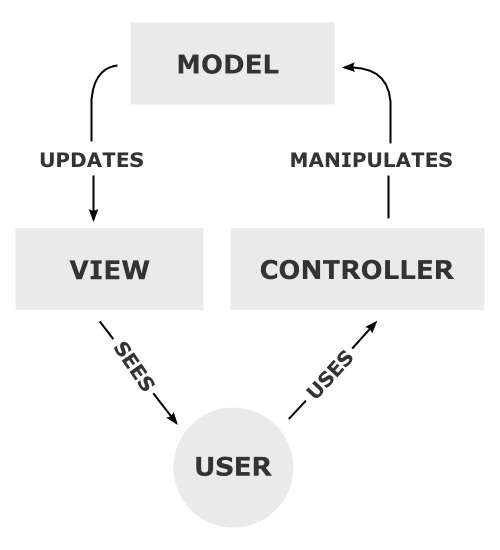
\includegraphics[width=.80\textwidth]{mvc.png}
    \caption{\footnotesize Model-View-Controller pattern}
    \label{fig:mvc}
\end{figure}

Using the model view controller pattern we can easily change the look and feel of the graphical user interface without interfering with how the model is updated. This gives a lot of freedom to continuously modify and improve the graphical user interface during the development of the application. 

\subsection{Package structure}
Using the discussed patterns as a basis, the following package diagram shown in figure~\ref{fig:packageDiagram}. 

\begin{figure}[h!]
  \centering
    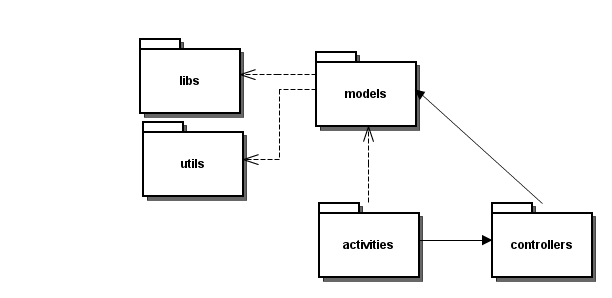
\includegraphics[width=.80\textwidth]{packageDiagram.png}
    \caption{\footnotesize Package diagram}
    \label{fig:packageDiagram}
\end{figure}

\begin{description}
	\item[libs] Contains the library classes used by the project. Currently only contains the java.swing.event.EventListenerList, which is used by Motea. This class is not included in the standard android packages because swing is not part of android.
	\item[utils] The modified Motej library (Modea), our implementation of the MadgwickAHRS algorithm resides here. Motea generates sensor events, and the MadgwickAHRS algorithm is used to calculate orientation.
	\item[modles] Classes holding the state of the Wii remote are contained here.
	\item[activites] Holds the Android activitiy classes. The MainActivity class starts the application and handles Android activity events. The CubeView class is used to generate a 3D-model illustrating the orientation of the connected Wii remote.
	\item[controller] Contains controller classes for interacting with the models and the Wii remote.
\end{description}

\subsection{Activity diagram}
The current application was created to be a proof of concept for the use of Wii remotes in fall detection/prevention applications. Figure~\ref{fig:activityDiagram} displays the basic functionality implemented in the solution. In addition to the 3D model that graphically displays the orientation of the Wii remote, an alarm system was also implemented. This alarm system is activated when the Wii remotes angle is greater than some predefined threshold. This threshold, is as of now, not customizable from the application itself but is hard-coded  into the application for now. 

The alarm uses sound and vibration to notify the user that the Wii remote angle has broken the threshold. Both sound and vibration is given in pulses with a delay between them, as the Wii remote angle becomes grater the delay between each pulse decreases. For the vibrotactile feedback the Wii remotes rumblepack is used and the sound is generated by the Android smartphone speaker. 


\begin{figure}[h!]
  \centering
    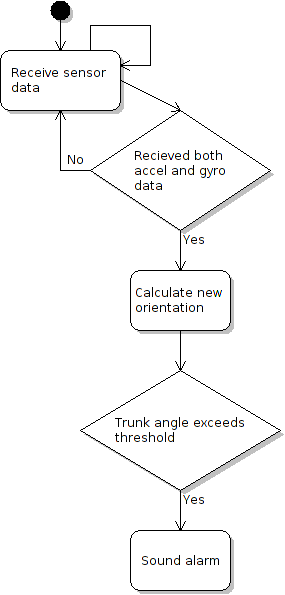
\includegraphics[width=.40\textwidth]{activityDiagram.png}
    \caption{\footnotesize Package diagram}
    \label{fig:activityDiagram}
\end{figure}

\subsection{Class diagram}
Figure~\ref{fig:classDiagram} shows a class diagram of the application's most important classes. The different background colors represents different parts of the system.

The classes with the red background handles the connection to the Wii remote. When the MainActivity class receives a BluetoothDevice object, that object is used to create an instance of Mote. The Mote class connects to the Wii remote. Each second the CheckStatus class is run to get an update about the Wii remotes battery life as well as trying to connect to the MotionPlus, if it is not already connected. The MotionPlus parses the extesion bytes recieved from the Wii remote, it also handles the manual calibration of the gyroscope.

The green background contains the controller classes. WiiMoteHandler handles all communication with the Motea classes (red background). It listens to both the accelerometer and gyroscope events from the Mote instance. When both an acceleromter event and a gyroscope event has been received the WiiMoteHandler WiiRemoteHandlerfires a sensor events. WiiMoteHandler also listens to alarm events to start the rumble pack in the Wii remote when the alarm goes off. Since this class is the only one talking to the Motea classes, this is the only class that needs major changes if it is decided to replace the Wii remotes with other types of sensors. 

AngleCalc listens to sensor events from the WiiMoteHandler, the gyroscope and acceleromter data are used to compute the orientation of the Wii remote and the trunk that it is straped to. To compute the orientation AngleCalc uses Madgwick's altitude and heading reference system algorithm, which is implemented in the MadgwickAHRS class. AngleCalc then updates the OrientationModel with the newly calculated orientation.

The yellow zone holds the models. OrientationModel hods the current orientation of the Wii remote and then fires an event when it is changed. A very simple noise canceling system has also been implemented here, to reduce the yaw drift when the Wii remote was kept still. Since the yaw rotation is will not be in the actual fall detection/prevention, this functionality is mainly to make the 3d cube model look better.

ThresholdAlarm listens to orientation events fired by the OrientationModel and then calculates whether the angle of is great enough to fire an alarm event. Alarm events have a severity variable that indicates how great the angle is. In the current implementation this variable is used to reduce the delay between rumble pulses and sound beeps, the greater the angle the faster the beeps.

The views have a blue background. MainAcitivty is the class that starts the application. It also handles Bluetooth discovery and initiates the appropritate classes when a Wii remote is detected. CubeView listens to the orientation evnets from the OrientationModel to crate a graphical representation of the position of the Wii remote. AlarmSound handles playing beeps from the smartphone when the ThresholdAlarm fires alarm events. 

\begin{figure}[h!]
	\centering
	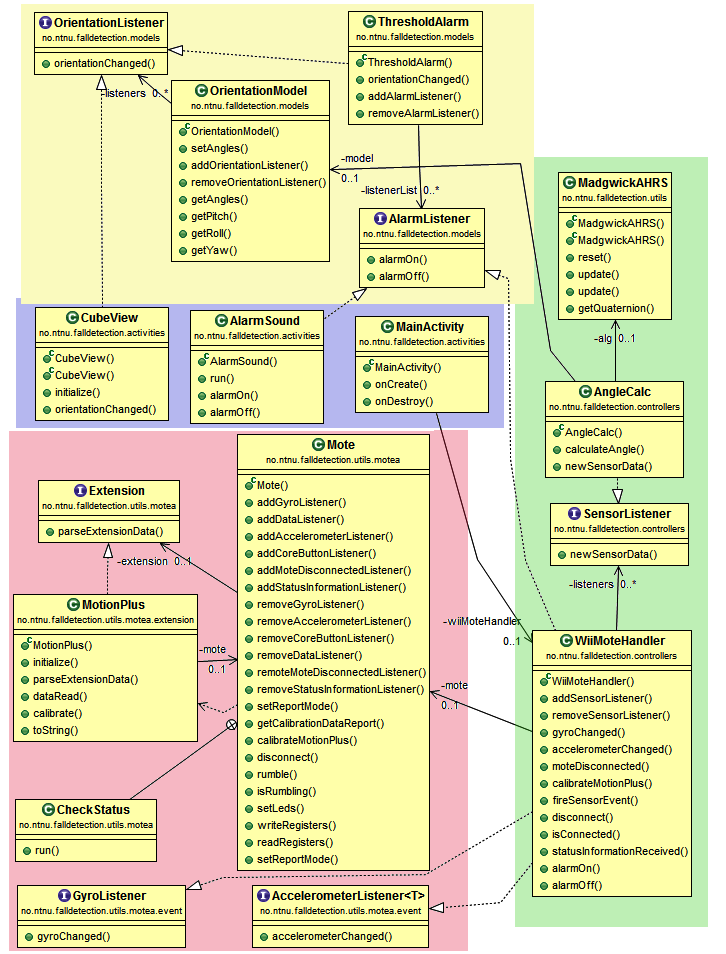
\includegraphics[width=1\textwidth]{classDiagram.png}
	\caption{\footnotesize Class diagram}
	\label{fig:classDiagram}
\end{figure}

\section{Limitations}
%Se på dette avsnittet knut. Tror hele må skriver på nytt hvor avsnittene under er merget og forklart bedre
The majority of Android devices have built-in Bluetooth cards, but the current Android SDK does not offer low level support for the Bluetooth stack, including L2CAP. This constraint can be bypassed on some devices by using reflection to access the socket constructor\cite{l2capHtc}. Access could also be gained through using the Android NDK (Native Develeoper Kit) but this is outside of our scope. Due to L2CAP not being official supported, certain vendors of Android devices have removed the L2CAP protocols completely, meaning that it would be impossible to use their Android OS to connect to the Wii Remote. Therefore the Android OS on the HTC Desire HD was altered to run with CyanogenMod 7 instead of the default HTC Sense.

Motej uses the BlueCove library as a multi-platform interface to the Bluetooth stack. Unfortunately, BlueCove does not support the Android OS. Android comes with its own Bluetooth API, the Android Bluetooth API. This means that the library will have to be re-written to work on the Android OS and support for the MotionPlus will have to be implemented. WiiMoteLib\cite{wiiMoteLib} is a C\# library which has support for the MotionPlus, by looking at the solutions in this library it should reduce the time required to implement MotionPlus support for the Motej library.

\section{Motej and Motejx}
The most complete of the Java based Wii remote libraries that could be found was Motej. Work on the library was discontinued in 2009, but supports all the main Wii remote functionality, and most of the extensions. It was therefore decided to use Motej as the base for a Wii remote library for Android. 

Figure~\ref{fig:moteClassDiagram} shows the most important classes of the Motej and Motejx libraries. To use the library you would create an instance of the Mote object, which takes care of handling the connection to the Wii remote. The Mote constructor takes a string with the bluetooth address of the Wii remote to connect to as input. It is also possible to use the MoteFinder class to discover any Wii remotes that are broadcasting for a connection. The Motej instance fires events whenever it receives data from the Wii remote it fires events that can be listened to by implementing the different listeners in the motej.events package. 

Wii remote exentions are handled by the Motejx library, which is an extension to the Motej library. All supported exensions have to be added to a extensions.properties file, which contains the extension id and the class that handles that type of exension. This way Motej does not need to know about any of the differnt extension implementations in the Motejx library. All extensions implement the Extension interface. To get data from the Wii remote extensions a listener has to be added to the extension class of that Wii remote extension.

%Add class diagram of motej and motejx

\section{Motej on Android}
For Motej to work on Android the BlueCove library has to be replaced with the Android Bluetooth API. This presents a major problem. Wii remotes uses the low level Bluetooth protocol L2CAP to connect to different platforms. As of Android version 4.1, Jelly Bean, \cite{jellyBean} there is no official support for L2CAP. Android only has full support for the higher level protocol \emph{radio frequency communication} (RFCOMM). RFCOMM is built on top of the L2CAP protocol and provides serial port emulation. 

Though the L2CAP is not directly supported through the Android Bluetooth API it is possible to create an L2CAP socket using a technique called reflection.

\begin{lstlisting}
Class<BluetoothSocket> cls = BluetoothSocket.class;
Constructor<BluetoothSocket> constructor = cls.getDeclaredConstructor(
		int.class, int.class, boolean.class, boolean.class,
		BluetoothDevice.class, int.class, ParcelUuid.class);

int type = 3, fd = -1, port = 0x13;
boolean auth = false, encrypt = false;
// Get some device
BluetoothDevice device = getBluetoothDevice();
ParcelUuid uuid = null;

/* type    - Type of socket (3 for L2CAP)
 * fd      - File descriptor (-1 for new socket)
 * auth    - Require authenticaton
 * encrypt - Require encrypted connection
 * port    - Remote port
 * uuid	   - SDP UUID
 */
// This will crate an L2CAP socket on port 0x13
BluetoothSocket socket = constructor.newInstance(type, fd, auth,
		encrypt, device, port, uuid);
\end{lstlisting}

This method has limitations. Because there is no official support for L2CAP in Android, many vendors roms will throw errors when trying to Bluetooth devices this way. Major vendors such as HTC and Samusng does, as of now, not support L2CAP connections.

\section{Motion Plus Support}
Motej has support for most of the common extensions for the Wii remote. Unfortunately Motion Plus is not one of the supported extensions. Motion Plus was implemented using the already existing extension structure of the Motej library.

Information on how to parse the incoming bytes from the Wii Remote was found on the WiiBrew wiki \cite{wiiBrew}. The date format is shown in figure~\ref{fig:motionPlusDataFormat}.

\begin{figure}[h!]
  \centering
    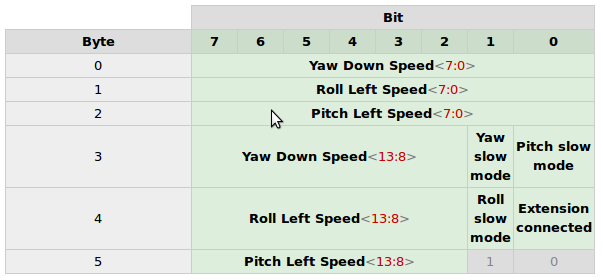
\includegraphics[width=.80\textwidth]{motionPlusDataFormat.png}
    \caption{\footnotesize Motion Plus data gyroscope data format}
    \label{fig:motionPlusDataFormat}
\end{figure}

\begin{lstlisting}
boolean yawFast = ((extensionData[3] & 0x02) >> 1) == 0;
boolean rollFast = ((extensionData[4] & 0x02) >> 1) == 0;
boolean pitchFast = ((extensionData[3] & 0x01) >> 0) == 0;

float yaw = 
	(extensionData[0] & 0xff | (extensionData[3] & 0xfc) << 6);
float roll = 
	(extensionData[1] & 0xff | (extensionData[4] & 0xfc) << 6);
float pitch = 
	(extensionData[2] & 0xff | (extensionData[5] & 0xfc) << 6);
\end{lstlisting}

An additional class was added for manual calibration of the gyroscope. There is calibration data stored in the Wii remote memory, but WiiBrew states that how to use these data for calibration is still unknown. Some suggestions on how to use the data exist, however the calibrated values are not very accurate compared to the manual calibration method. During manual calibration it is required that the Wii remote is kept still. The calibration takes less than 1 second.

%Trenger ikke vente på ack så lenge man bruker den data pipe for å send forespørsler.
%When implementing Motion Plus support, another weakness in the Motej library was discovered. After the Motion Plus extension has been connected to the Wii remote, the new data is not sent automatically. To receive the data, the report mode has to be changed. The report mode tells the Wii remote what data to send back to the device it is conneted to. To change the report mode you have to send a some specific bytes to the Wii remote. This functionality is already implemented in Motej, however the library did not check for the message to be received by the Wii remote before allowing new commands to be sent. Because of this, changing the report mode right after initializing the extension was not detected by the Wii remote.

\subsection{Orientation}
A major disadvantage with the Wii Remote compared to competing gaming peripherals such as PS Move and Kinect is that the data output is always relative to itself. In other words, the Wii Remote does not say anything about where it is located in space. Even though the Wii Remote does not provide its orientation out of the box, the data it does provide is enough for developers to calculate the orientation of the Wii Remote. Calculating the orentation of the Wii requires dedicated algorithms that used advanced mathematical formulas. Calculations are performed on the sensor data collected from the Wii Remote and Motion Plus extension. The accelerometer data enables developers to determine the tilt of the Wii Remote while gyroscope data allows developers to determine the movement speed in three directions. Only by utilizing both can the algorithms calculate the orientation of the Wii Remote.

We chose to use the Madgwick algorithm\cite{madgwick}. This choice was based on the fact that a master thesis by Tryggestad\cite{Tryggestad} had used the same algorithm for Wii Remote orientation successfully. A C\# implementation of the algorithm is available at the x-io Technologies Limited website \cite{opensourceMadgwick}, we used this as a basis for the Java implementation of the algorithm which is used in our application. The constructor of the algorithm requires two parameters a sample periode and an algorithm gain beta. The sample period was set to 1f/100f and the algorithm gain beta was set to 0,5f. Sample periode is equal to the refresh rate of the Wii Remote and the beta is based on findings by Tryggestad. These values proved to be satisfactory for us as well.

\begin{figure}[h!]
  \centering
    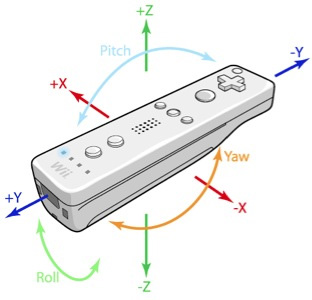
\includegraphics[width=.45\textwidth]{wiimoteAxis.png}
    \caption{\footnotesize A visual representation of the cartesian coordinate system for the Wii Remote, taken from Wii Brew\cite{wiiBrew}.}
\end{figure}

% Sette algoritmen i appendix?

The algorithm update method requires six parameters: The first three are the gyroscope's X, Y, and Z axis measurements provided in radians/, the following three are the accelerometers X Y Z in any calibrated unit. We discovered that what is defined as yaw, pitch, and roll is not universal, and which axis each corresponds to might be different for aviation and gaming controllers. Rotation about the X axis corresponds pitch, Y corresponds roll and Z corresponds to yaw such as shown in % REF TO IMAGE
The algorithm returns the result as a Quaternion that need to be stored and converted to Euler angles. The formulas for converting the Quaternion to Euler angles are provided in the Madgwick paper. The formula for roll is incorrect in the paper, providing us with incorrect values, Tryggestads calculation was used for the roll conversion. The change was minor as Madgwick uses the wrong quaternion unit for roll calculation.

%SHINY PICTURZS OF OUR CODE

\section{Motea}
During the modification of the Motej library it soon became apparent that several parts of the library were outdated or not optimal for the current application. One problem was discovered when implementing rumbling response to alarm events. The rumble pack was turned off each time a request for status information was sent to the Wii remote. This bug was caused by the fact that Motej did not modify the status information request with the current status of the rumble pack.

It was also discovered that Motej used an outdated port to send requests to the Wii remote. Motej used the control pipe with report 0x52 to send requests. This method only works for the original Wii remotes, and will not work for the newer models. During testing the original Wii remote with external MotionPlus was used and therefore this problem was not discovered before later in the development phase.

Because of all the small bugs and the large portions of the library that were not used it was decided to create a lightweight Wii remote library from scratch. The new library was based on the general structure of Motej, and some of the code was also reused. Motea uses the data pipe for both sending and receiving data from the Wii remote. This way the new library should suppor the newer Wii remotes. 

Currently these input report modes are supported:
\begin{description}
	\item[0x20] Status information
	\item[0x21] Read memory and registers
	\item[0x37] Core buttons, acceleromter, extension data (gyroscope)
\end{description}

Report mode 0x37 also contains bytes with data from the IR camera, but this functionality was not needed and therefore not added to the Motea library.

Supported output reports are:
\begin{decription}
	\item[0x11] Set LEDs and activate rumble pack
	\item[0x12] Sed data report mode (only 0x37 will be used)
	\item[0x15] Status information request
	\item[0x16] Write to memory and registers (used for activating MotionPlus)
	\item[0x17] Read memory and registers (for calibration reports)
\end{description}

The new library has working support for rumbling and connecting the MotionPlus extension while rumbling, which also was problematic with Motej. Motea also sends requests for status information and checks for MotionPlus (if not connected) each second. This way any class listening to status information events get regular updates, and not just when an extension is connected.